\section{Measured results}
\label{sec:results}
The following results come from the frozen comparison defined in Section~\ref{sec:design}. Table~\ref{tab:reconstruction-times} gives completion and elapsed time by physical structure. Each time is a sum of per-request medians on the same completed inputs for both methods.
\begin{table}[!htbp]\centering\small
\caption{Current application versus the preceding application with direct vacuum formulas. Done gives preceding/integrated completions; paired gives the number completed by both.}
\label{tab:reconstruction-times}
\begin{tabularx}{\linewidth}{@{}Yrrrr@{}}\toprule
Domain & Done & Paired & Preceding (s) & Integrated (s)\\\midrule
Connected trees, 1--13 loops & 34/34 & 34 & 5.839 & 5.788 \\
Zero-invariant tensors & 3/3 & 3 & 0.596 & 0.602 \\
Ordinary one-loop tensors & 3/3 & 3 & 0.731 & 0.728 \\
Vacuum products, 1--13 loops & 13/13 & 13 & 2.147 & 2.132 \\
Two-loop planar boxes & 9/9 & 9 & 18.206 & 11.360 \\
Two-loop nonplanar boxes & 9/9 & 9 & 45.732 & 23.320 \\
Two-loop massive sunrise & 2/2 & 2 & 2.658 & 2.439 \\
Three-loop massive vacuum & 2/2 & 2 & 3.713 & 3.482 \\
All 75 requests & 75/75 & 75 & 79.624 & 49.852 \\
\bottomrule\end{tabularx}\end{table}

The integrated-to-preceding ratio is 0.626, with central 95\% request-resampling interval $[0.485,0.816]$. Its point estimate corresponds to 37.4\% less time. The integrated application is slower on 29 matched requests. These are complete application times, so the reduction includes the cost of loading and choosing the method.

\subsection{Native algebra and learned selection}
The 22 matched native requests change from 70.310 to 40.602 seconds, a ratio of 0.577 with interval $[0.420,0.774]$. The selected finite-field reconstruction is an established Kira capability. Its effect must be separated from the model that selects its settings.

Training uses 48 verified requests and validation uses 22. Validation selects maximum tree depth 4, minimum leaf population 2, and saving margin 0.05. The selected model gives 47.615 seconds of validation cost, compared with 48.173 seconds for the structure-dependent fixed control. This does not satisfy the deployment condition, so the integrated application uses the validated fixed settings. The fitted model and its measurements are preserved, and its weights are not loaded for production decisions.

On the reserved native sample, the fixed application takes 40.274 seconds and the integrated application takes 40.602 seconds. Their ratio is 1.008, with interval $[0.999,1.018]$. Both applications use the same selected settings, so their difference measures run-to-run variation and the shared entry procedure. It is not an added ML speedup. The final repetition changes 0 of 22 actions relative to the fixed control. The feature-range guard sends 3 requests to the preceding symbolic procedure. Median configuration-loading and decision time is 105.779 milliseconds, including the first loading of the feature dependencies. This quantity is not pure forest evaluation time. The preceding seed model remains shared by both applications.

\begin{figure}[!htbp]\centering
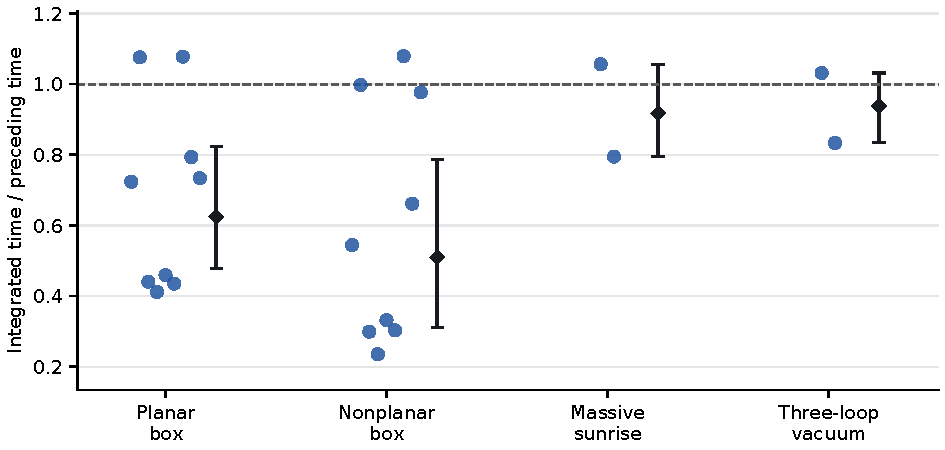
\includegraphics[width=.97\linewidth]{paper_figures/reconstruction_native.pdf}
\caption{Native speed changes depend on the physical request. Each circle shows the integrated-to-preceding ratio for one completed request. Diamonds show ratios of summed median times within each structure, with paired request-resampling intervals. Values below one mean less elapsed time.}
\label{fig:reconstruction-native}
\end{figure}
\begin{figure}[!htbp]\centering
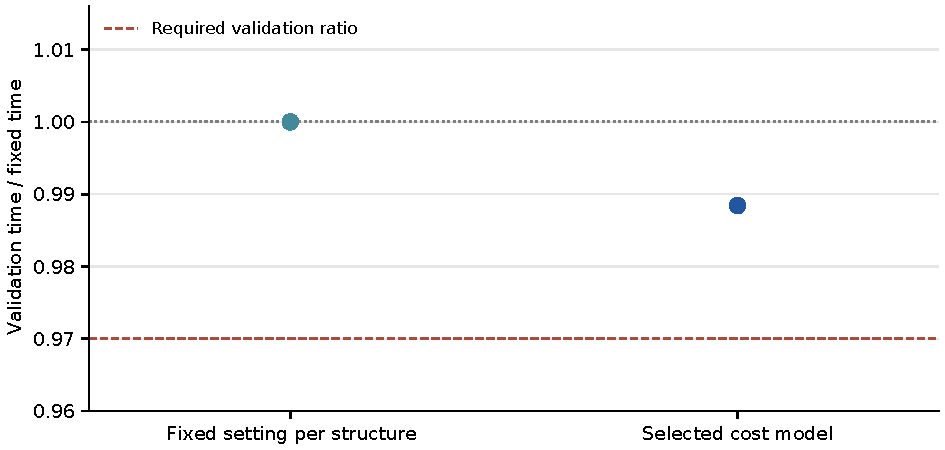
\includegraphics[width=.97\linewidth]{paper_figures/reconstruction_ml.pdf}
\caption{Separate validation determines whether the new model is used. The dashed threshold requires at least three percent less cost than the fixed setting selected for each structure. The current deployment retains the fixed settings because the model does not meet this condition.}
\label{fig:reconstruction-ml}
\end{figure}

\subsection{Cumulative change and exact reductions}
The matched comparison across the last two extensions changes from 81.827 to 49.852 seconds on 75 completed requests. Its ratio is 0.609, with interval $[0.470,0.787]$, or 39.1\% less time at the point estimate. This result uses one input set and one timing procedure. It is a cumulative comparison with the earlier application, not with unmodified Kira, and it does not multiply percentages from older experiments.

The direct vacuum formulas and connected-tree recurrences remain active through thirteen loops. They provide rational master decompositions and explicit Gamma-function values in the domains derived in the appendices. The present analytic grid verifies their preservation while the new algebra method changes the native calculations. General coupled multiscale scattering through thirteen loops is outside this grid.
\begin{figure}[!htbp]\centering
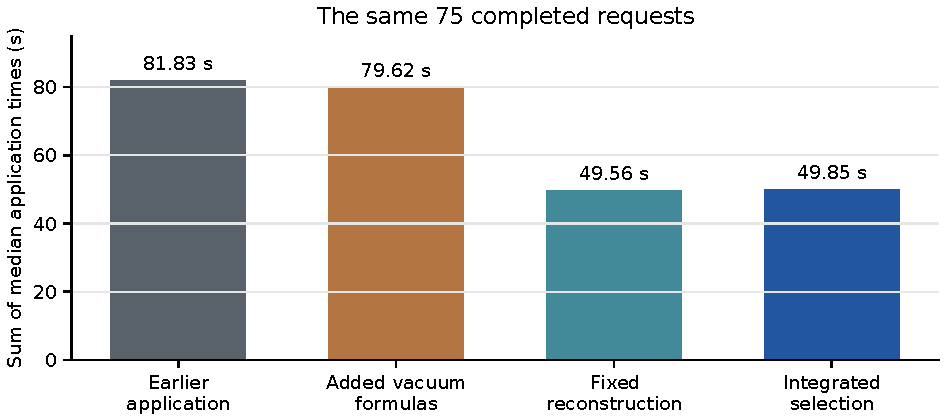
\includegraphics[width=.97\linewidth]{paper_figures/reconstruction_components.pdf}
\caption{Cumulative elapsed time is measured on the same requests for all four applications. The second application adds direct vacuum formulas; the third adds validated fixed reconstruction settings; the fourth applies the admitted selection procedure. The bars do not combine unrelated historical speed factors.}
\label{fig:reconstruction-components}
\end{figure}
\begin{figure}[!htbp]\centering
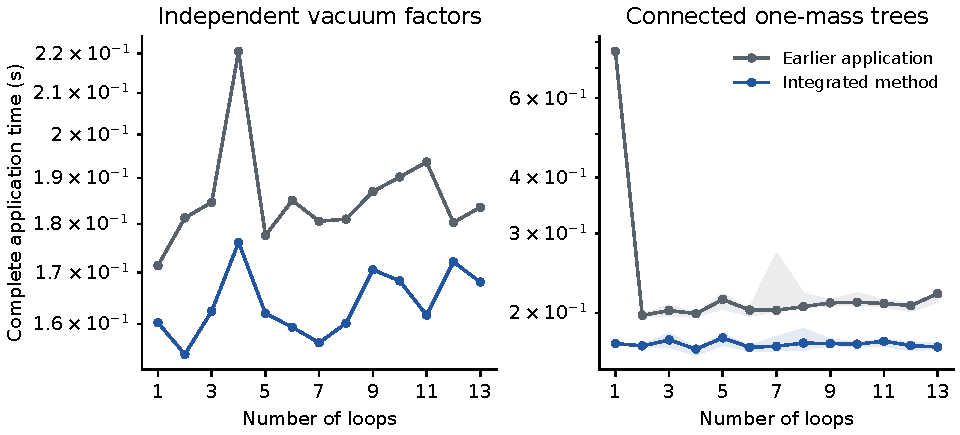
\includegraphics[width=\linewidth]{paper_figures/reconstruction_exact.pdf}
\caption{The analytic stage covers each loop order from one through thirteen in its stated domains. The left panel shows independent vacuum factors. The right panel shows connected one-mass trees, with the median over available shapes and their full range. Logarithmic time axes show the small complete application times without hiding their variation.}
\label{fig:reconstruction-exact}
\end{figure}
\subsection{Completion and scope}
The timed outputs receive 18,132 exact coefficient comparisons. The integrated application has 0 unverified timed applications and 0 recorded unsuccessful inner native attempts. It uses reconstruction recovery 0 times. Reference preparation fails for 0 final requests. Application failure counts include a terminated run even when it cannot return an inner-attempt record.

The current native test measures new kinematic points and complete target batches within four known structures at two and three loops. Higher-loop evidence comes from the derived product and tree identities. It does not establish performance for every high-loop graph, every symbolic kinematic system, or unrestricted numerator powers. The measured configuration also depends on the tested processor and resource bounds. A finite model and setting search does not prove globally minimum time.
\subsection{Retained ML in the reconstruction workflow}
The additional paired comparison holds the new algebra settings fixed and switches the inherited learned choices to their existing fixed procedure. On 22 matched native requests, the fixed procedure takes 42.175 seconds and the learned procedure takes 41.448 seconds. Their ratio is 0.983, with interval $[0.951,1.003]$. This interval includes equal time, so the sample does not resolve a consistent additional learned saving. The recorded seed-attempt sequences differ on 14 requests. The learned and fixed procedures have 0 and 0 unverified applications, respectively. Across all three repetitions, their total times are 128.032 and 127.546 seconds. The distinction between total repeated time and summed medians illustrates the timing variation. This ablation has its own paired timings; its ratio is not multiplied into the cumulative result.

\begin{table}[!htbp]\centering\small
\caption{Inherited learned choices versus their existing fixed procedure, with the new reconstruction settings shared. The columns use matched completed requests within each structure.}
\label{tab:reconstruction-retained}
\begin{tabularx}{\linewidth}{@{}Yrrrr@{}}\toprule
Structure & Paired & Fixed (s) & Learned (s) & Ratio\\\midrule
Planar box & 9 & 11.656 & 11.482 & 0.985 \\
Nonplanar box & 9 & 24.355 & 23.842 & 0.979 \\
Massive sunrise & 2 & 2.565 & 2.542 & 0.991 \\
Three-loop vacuum & 2 & 3.600 & 3.582 & 0.995 \\
All native requests & 22 & 42.175 & 41.448 & 0.983 \\
\bottomrule\end{tabularx}\end{table}


\subsection{The other learned interventions}
Table~\ref{tab:retained-results} retains the main earlier controls needed to interpret the method. They use different workloads and cannot be multiplied into a cumulative speed factor. The equation-filter result supports that intervention on its tested domain, while the row results motivate its omission. The current combined experiment keeps equation filtering off and does not claim a joint seed-plus-equation gain.
\begin{table}[!htbp]\centering\small
\caption{Earlier measurements from this study, retained as separate evidence. A ratio below one means less time. Their full input definitions and measurements remain in the notes.}
\label{tab:retained-results}
\begin{tabularx}{\linewidth}{@{}YYr@{}}\toprule
Intervention & Control and workload & Time ratio\\\midrule
Earlier native seed model & Fixed region, 32 box batches: 156.383 to 150.663 s & 0.963\\
Equation selection & Native filter, 24 new-index batches: 72.295 to 67.478 s & 0.933\\
Original learned row model & Native row choices, 84 trials & 1.305\\
Compiled row-cost policy & Native row choices; geometric mean & 0.982\\\bottomrule
\end{tabularx}
\end{table}
The earlier seed comparison has interval $[0.937,0.984]$, and the equation comparison has interval $[0.928,0.940]$. The compiled row policy has interval $[0.959,1.003]$, which includes equal time. These intervals use the resampling procedure recorded for each original study. The native row algorithm remains in the retained workflow.

\FloatBarrier
